\documentclass{beamer}
\usetheme{default}

\usepackage[italian]{babel}
\usepackage[utf8x]{inputenc}

\usepackage{subcaption}

\title{Il percorso di una proposta dall'idea all'approvazione in programma, nel Partito~Pirata~Italiano}
\author{Giuseppe Cal.}
\institute{Partito Pirata Italiano -- Pirate Party of Italy}
\date{\today}

\begin{document}

\begin{frame}
\maketitle
\end{frame}

\begin{frame}{Sezioni ed aree}
LiquidFeedback 2.x divide il campo decisionale in sezioni (\emph{units}) ed aree: 
\begin{columns}
\begin{column}{0.5\textwidth}
\begin{itemize}
\item Una \emph{sezione} raggruppa insieme aree affini, come ad esempio, quelle relative all'amministrazione piuttosto che ai contenuti o alla produzione documentale.
\item Un'\emph{area} \`e un insieme pi\`u ristretto, utile a trattare in modo diverso gli affari esteri e la regolamentazione dei trasporti, nell'esempio.
\end{itemize}
\end{column}
\begin{column}{0.5\textwidth}
\begin{figure}
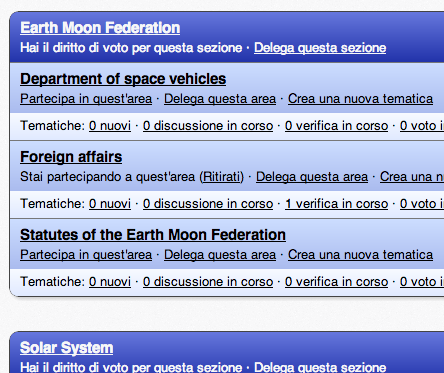
\includegraphics[width=0.95\textwidth]{pics/unitarea}
\caption{Le sezioni sulla federazione terra luna con le rispettive aree. Intravista, la sezione sul sistema solare.}
\end{figure}
\end{column}
\end{columns}
\end{frame}

\begin{frame}{Aree, ``interesse'' e quorum}
Per evitare che vengano discusse proposte poco interessanti, \`e richiesto che un certo numero di supporters portino avanti le proposte che ritengono interessanti.

Questo numero \`e regolabile per ogni area ed \`e proporzionale al numero di utenti che dicono---cliccando sull'apposito \emph{partecipa in quest'area}---di essere interessati ad un'area.
\begin{figure}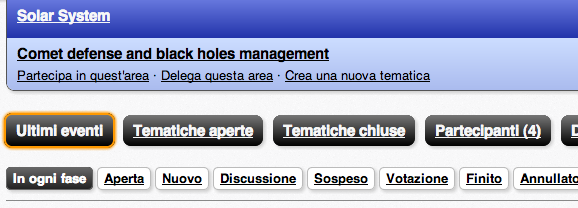
\includegraphics[width=0.8\textwidth]{pics/partecipa}
\caption{Come esprimere la propria ``partecipazione.''}
\end{figure}
\end{frame}

\begin{frame}{Aree e deleghe}
In alternativa alla partecipazione diretta, \`e possibile impostare un fiduciario che agir\`a in proprio nome all'interno di quell'area; o decidere di ignorarla del tutto, fidandosi di ci\`o che gli altri decidono. Di default, un'area eredita le impostazioni di delega della sezione che la contiene, ma \`e possibile scegliere in maniera granulare.
\begin{figure}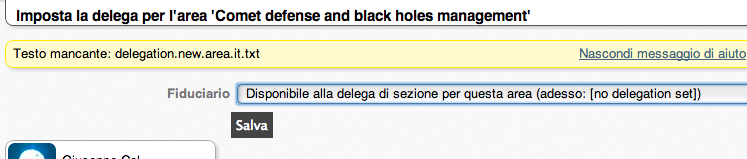
\includegraphics[width=0.8\textwidth]{pics/delega}
\caption{Deleghi qualcuno scegliendo fra i tuoi contatti e salvando.}
\end{figure}
\end{frame}

\begin{frame}{Seguire le aree}

Una volta scelte le aree che vogliamo seguire, torniamo alla home page. Da qui, cliccando su ``ultimi eventi'' possiamo vedere cosa succede nelle nostre aree preferite, ed anche in tutte le altre, giocando opportunamente con i filtri.
\begin{figure}
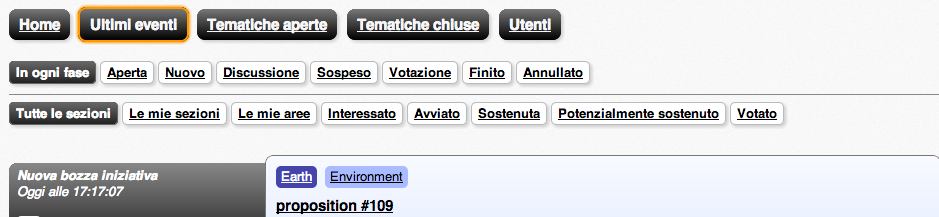
\includegraphics[width=0.99\textwidth]{pics/timeline-filters}
\caption{In alto, i filtri. In basso, gli eventi.}
\end{figure}
\end{frame}

\begin{frame}{Creare una nuova proposta... }
Hai avuto un'idea geniale per un punto che ancora manca nel programma del PP-IT, e vuoi che sia inclusa.

Nulla di pi\`u semplice: \begin{itemize}\item scegli l'area adatta;\item clicca su ``Crea una nuova tematica;''\item scrivi e salva.\end{itemize}
\begin{figure}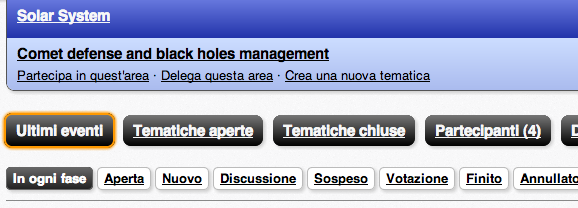
\includegraphics[width=0.8\textwidth]{pics/partecipa}
\caption{``Crea una nuova tematica''}
\end{figure}

\end{frame}

\begin{frame}{...o rispondere ad una gi\`a presente}
\begin{columns}
\begin{column}{.5\textwidth}Hai visto un'iniziativa. Ma non ti piace o vuoi comunque migliorarla. Bene, durante la fase di discussione hai due possibilit\`a:\begin{itemize}\item Scrivere un'alternativa: link apposito, quindi scrivi e salva; \item Suggerire un'emendamento, tassativo o meno. \end{itemize}\end{column}
\begin{column}{.5\textwidth}\begin{figure}\includegraphics[width=\textwidth]{pics/init}
\caption{``Crea un'iniziativa alternativa,'' ``Nuovo suggerimento''}
\end{figure}\end{column}
\end{columns}

\end{frame}

\begin{frame}{Discutere con i pirati}
Adesso hai presentato la tua iniziativa. C'\`e chi l'ha gradita e ti ha dato supporto, c'\`e chi ha suggerito emendamenti, c'\`e chi ha proposto un'antitetica alternativa. \begin{itemize}\item Le alternative ti fanno vedere in che modo i tuoi colleghi pirati affrontano lo stesso problema. \item I suggerimenti ti dicono che pensano della tua!\begin{itemize}\item {\bfseries Sono valutati}: per ogni suggerimento sai qual \`e il numero dei pirati favorevoli, nei due gradi, e quello dei contrari. \item \`E {\bfseries valutata anche la tua implementazione} del suggerimento.\end{itemize}\end{itemize} \begin{figure}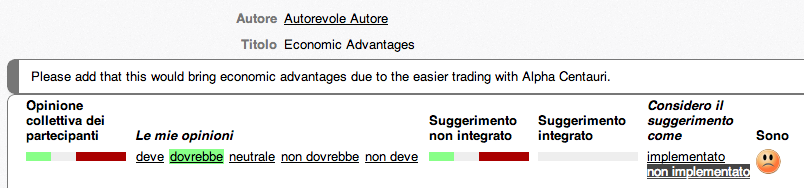
\includegraphics[width=\textwidth]{pics/suggerimento}
\caption{Un suggerimento nel dettaglio}
\end{figure}
\end{frame}

\begin{frame}{Votare}
Terminata la fase di discussione, la tematica entrer\`a in una fase di congelamento durante la quale sar\`a possibile soltanto leggere, dare/togliere supporto e presentare iniziative alternative di emergenza.

Tutte le iniziative che raggiungono un determinato quorum di supporto vengono presentate sulla scheda per il voto:\begin{itemize}\item Non \`e un semplice voto si/no oppure ``la mia preferita \`e questa.''\item Sulla scheda va espressa una classifica di gradimento delle proposte, ``questa \`e la mia preferita,'' ``questa andrebbe comunque bene,'' ``questa \`e brutta, ma quelle sotto sono peggio,'' ``questa mi fa completamente schifo.''\end{itemize}

\end{frame}

\begin{frame}{La scheda}
\begin{figure}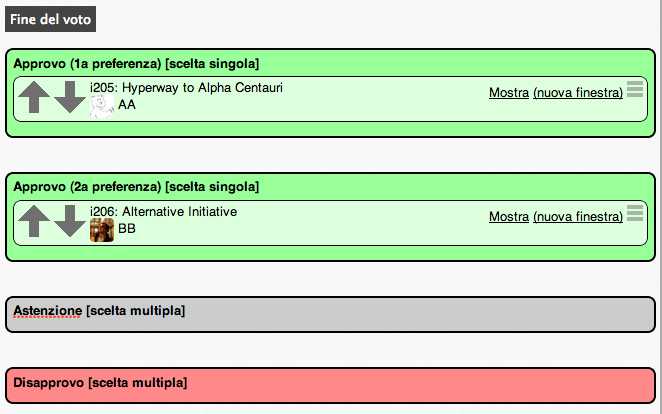
\includegraphics[width=.9\textwidth]{pics/scheda}
\caption{In basso, il pulsante per confermare il voto}
\end{figure}
\end{frame}

\begin{frame}{Metodo Schulze}
\begin{itemize}
\item Prende in ingresso gli ordinamenti delle schede e produce un ordinamento dei candidati, in modo che, se la maggior parte dei votanti ha preferito la proposta $A$ a quella $B$, la proposta $A$ sar\`a sopra la $B$ nell'ordinamento finale.
\item \`E a prova di clone: non c'\`e il problema che due proposte uguali si contendano i voti, perch\'e ogni votante pu\`o mettere pi\`u proposte nella stesa scatola, dichiarandosi indifferente fra le due.
\item {\bfseries La proposta che \`e preferita a tutte le altre arriva prima e vince}.
\end{itemize}
\end{frame}

\begin{frame}{Verificare i risultati}
Alla fine della fase di voto saranno disponibili ai votanti le schede di tutti, con l\`indicazione di chi ha votato cosa.

\begin{itemize}\item Questi dati sono utilizzabili per verificare che la macchina non imbrogli i votanti, scegliendo al loro posto.\end{itemize}
\begin{figure}
	\begin{subfigure}[b]{.58\textwidth}
		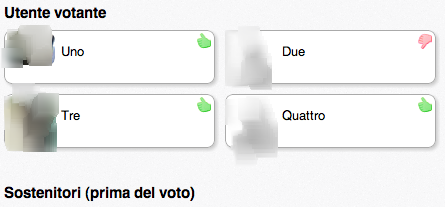
\includegraphics[width=\textwidth,]{pics/voters}
		\caption{Chi e come ha votato la proposta...}
	\end{subfigure}
	\begin{subfigure}[b]{.34\textwidth}
		\includegraphics[width=\textwidth]{pics/scheda-post}
		\caption{...in dettaglio}
	\end{subfigure}
\caption{Come vedere chi ha votato cosa.}
\end{figure}

\end{frame}

\end{document}
